\documentclass{article}
\usepackage{amsthm}
\usepackage{graphicx}
\usepackage{rotating}
%\makeatletter
%\def\note{\@ifnextchar[{\@noteWith}{\@noteWithout}}
%\def\@noteWith[#1]{\medbreak\refstepcounter{section}%
%  \renewcommand{\leftmark}{Lecture \thesection}
%  \noindent{\addcontentsline{toc}{section}{Note \thesection: #1\@addpunct{.}}%
%  \sectionfont Note \thesection. #1\@addpunct{.}}\medbreak}
%\def\@noteWithout{\medbreak\refstepcounter{section}%
%  \renewcommand{\leftmark}{Note \thesection}
%  \noindent{\addcontentsline{toc}{section}{Note \thesection.}%
%  \sectionfont Note \thesection.}\medbreak}
%\makeatother

\title{Bellarmine 2017 Eclipse Plans and Notes}

\author{Stephen Brown and Ahktar Mahmood}
\begin{document}

\maketitle


\section{Notes given to us}

\begin{itemize}
\item Provide expert perspective about the upcoming solar eclipse
\item ``How to watch the eclipse"
\item A description of what's happening in the sky
\item What has everyone so excited about this particular opportunity,etc.
\end{itemize}


\section{Stephen's notes}

\subsection{Understand!}
MUST BE IN SHADED REGION TO SEE TOTALITY!
\begin{figure}[h]
\centering
\includegraphics[width=85mm]{Pictures/usa_eclipse_map_v2.jpg}
\caption{Total Eclipse Map of United States}
\end{figure}

\begin{figure}[h]
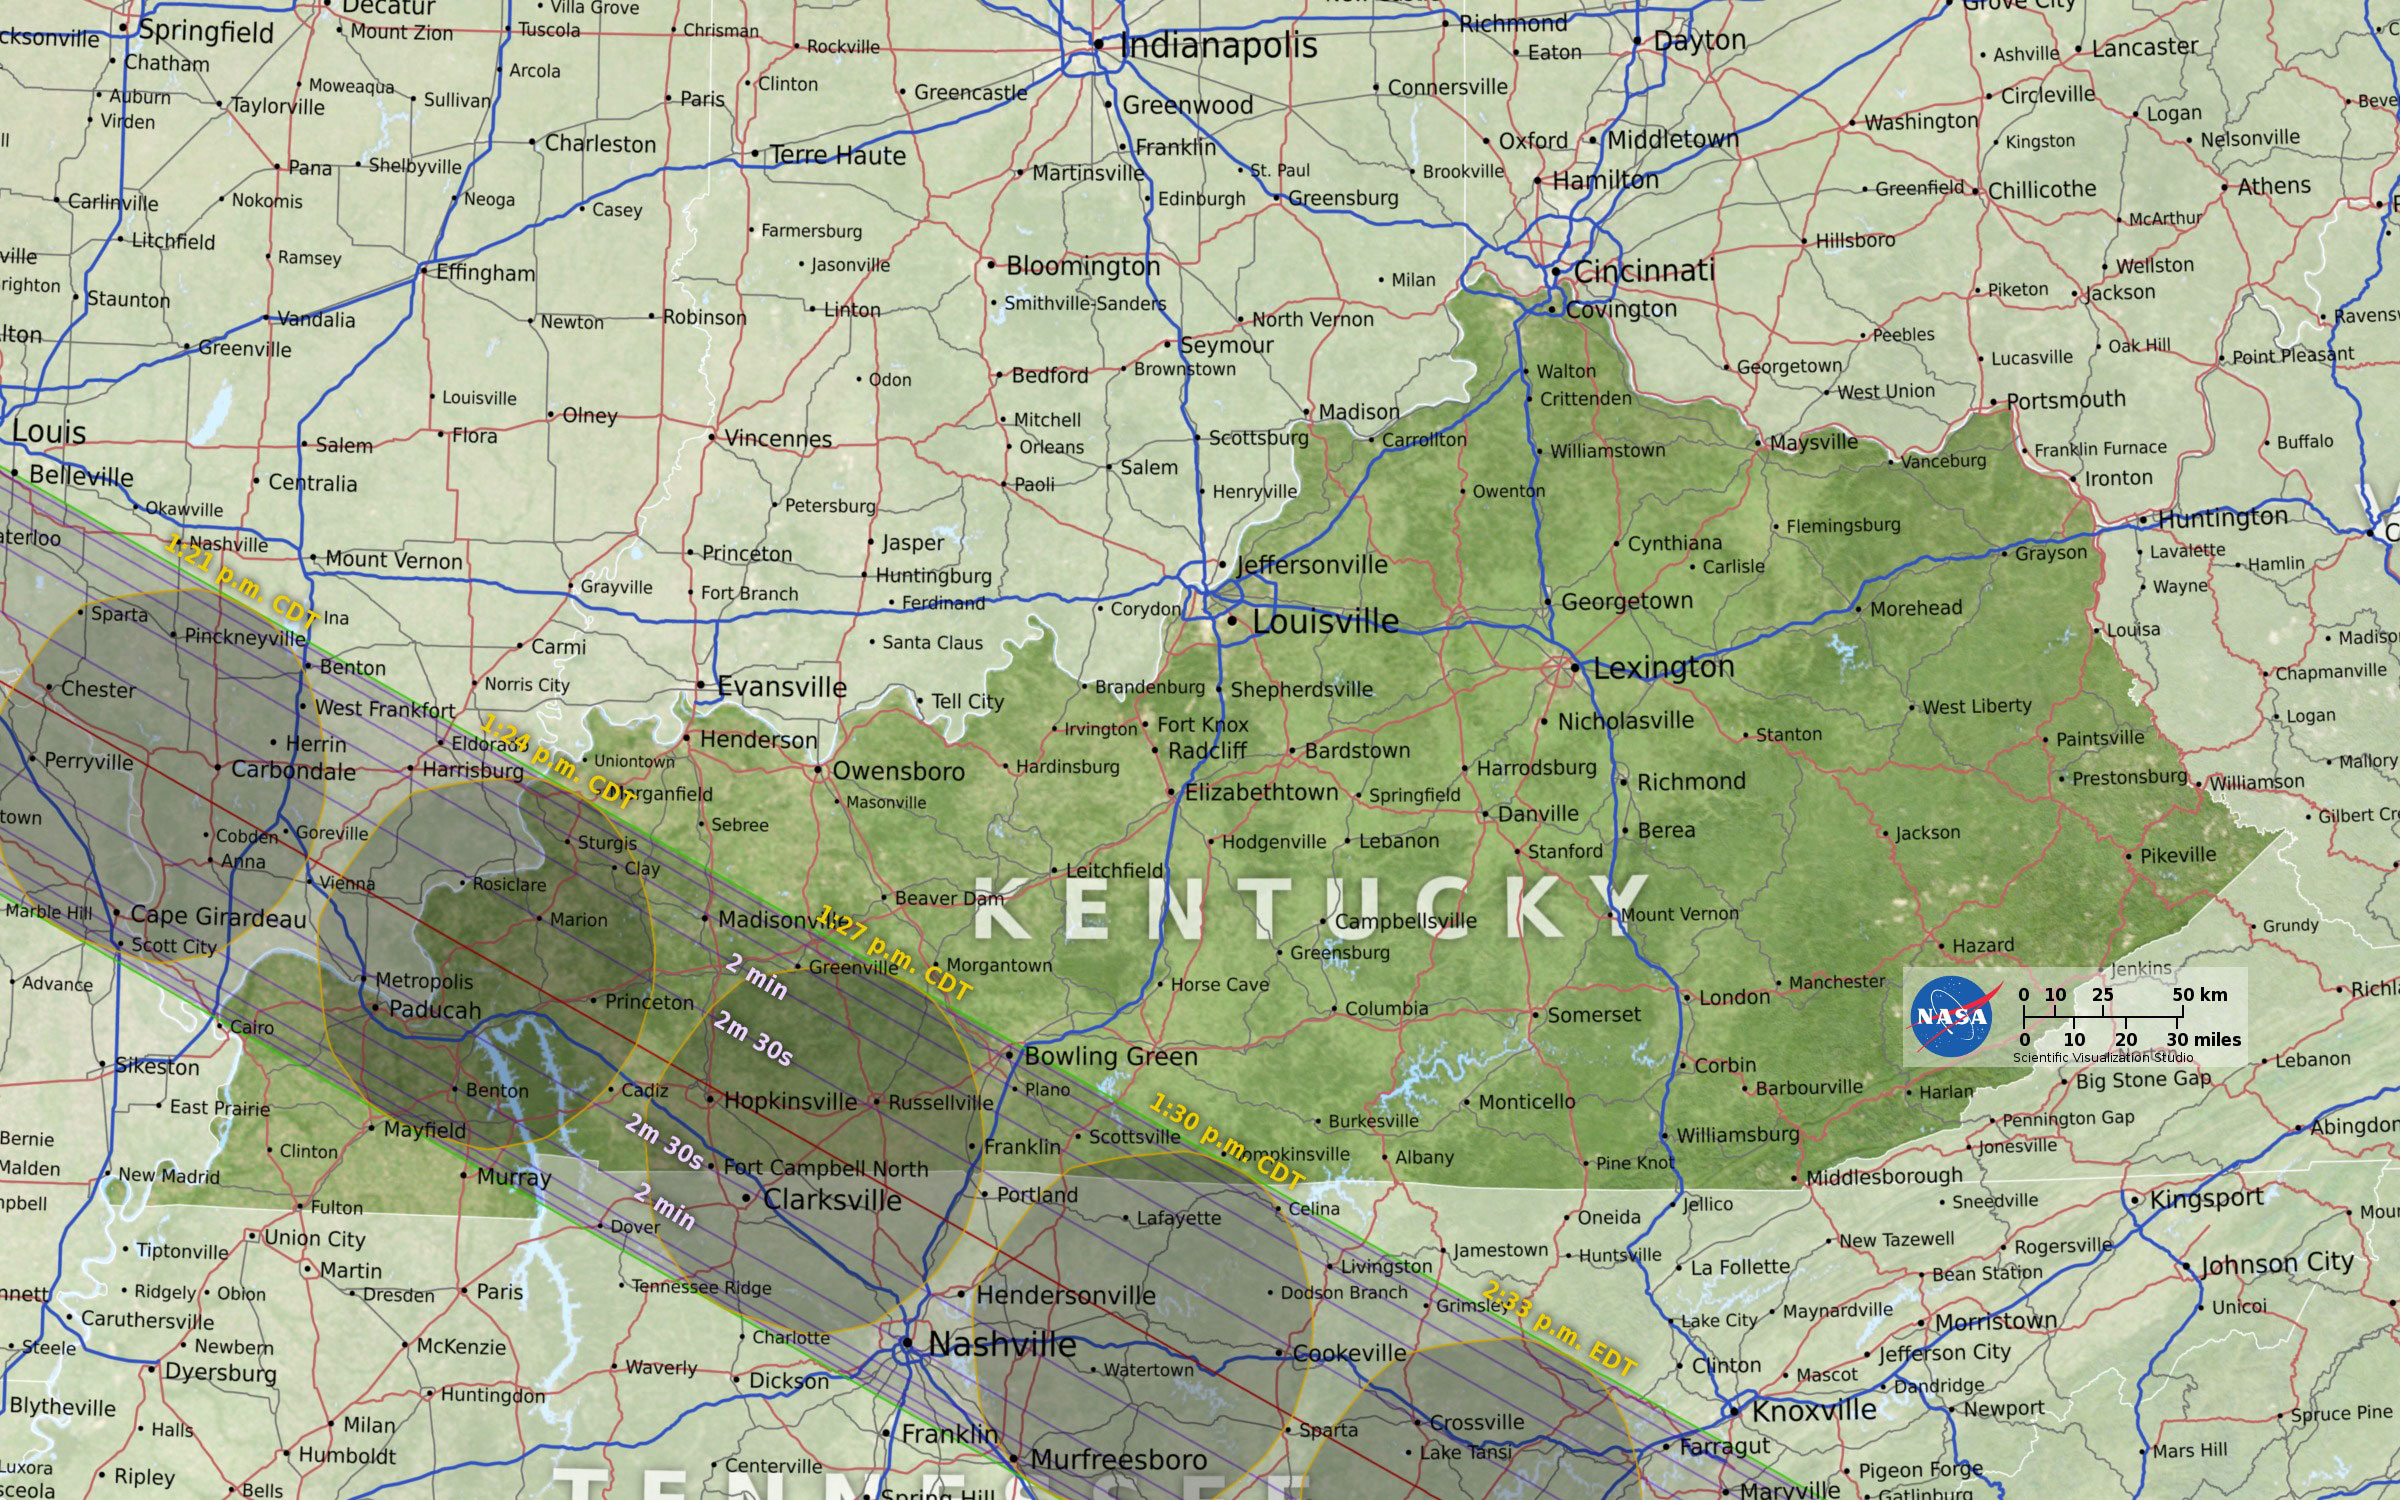
\includegraphics[scale=.2]{Pictures/Ky_eclipse_path.jpg}
\caption{Kentucky's Path of Totality}
\end{figure}

\begin{sidewaysfigure}
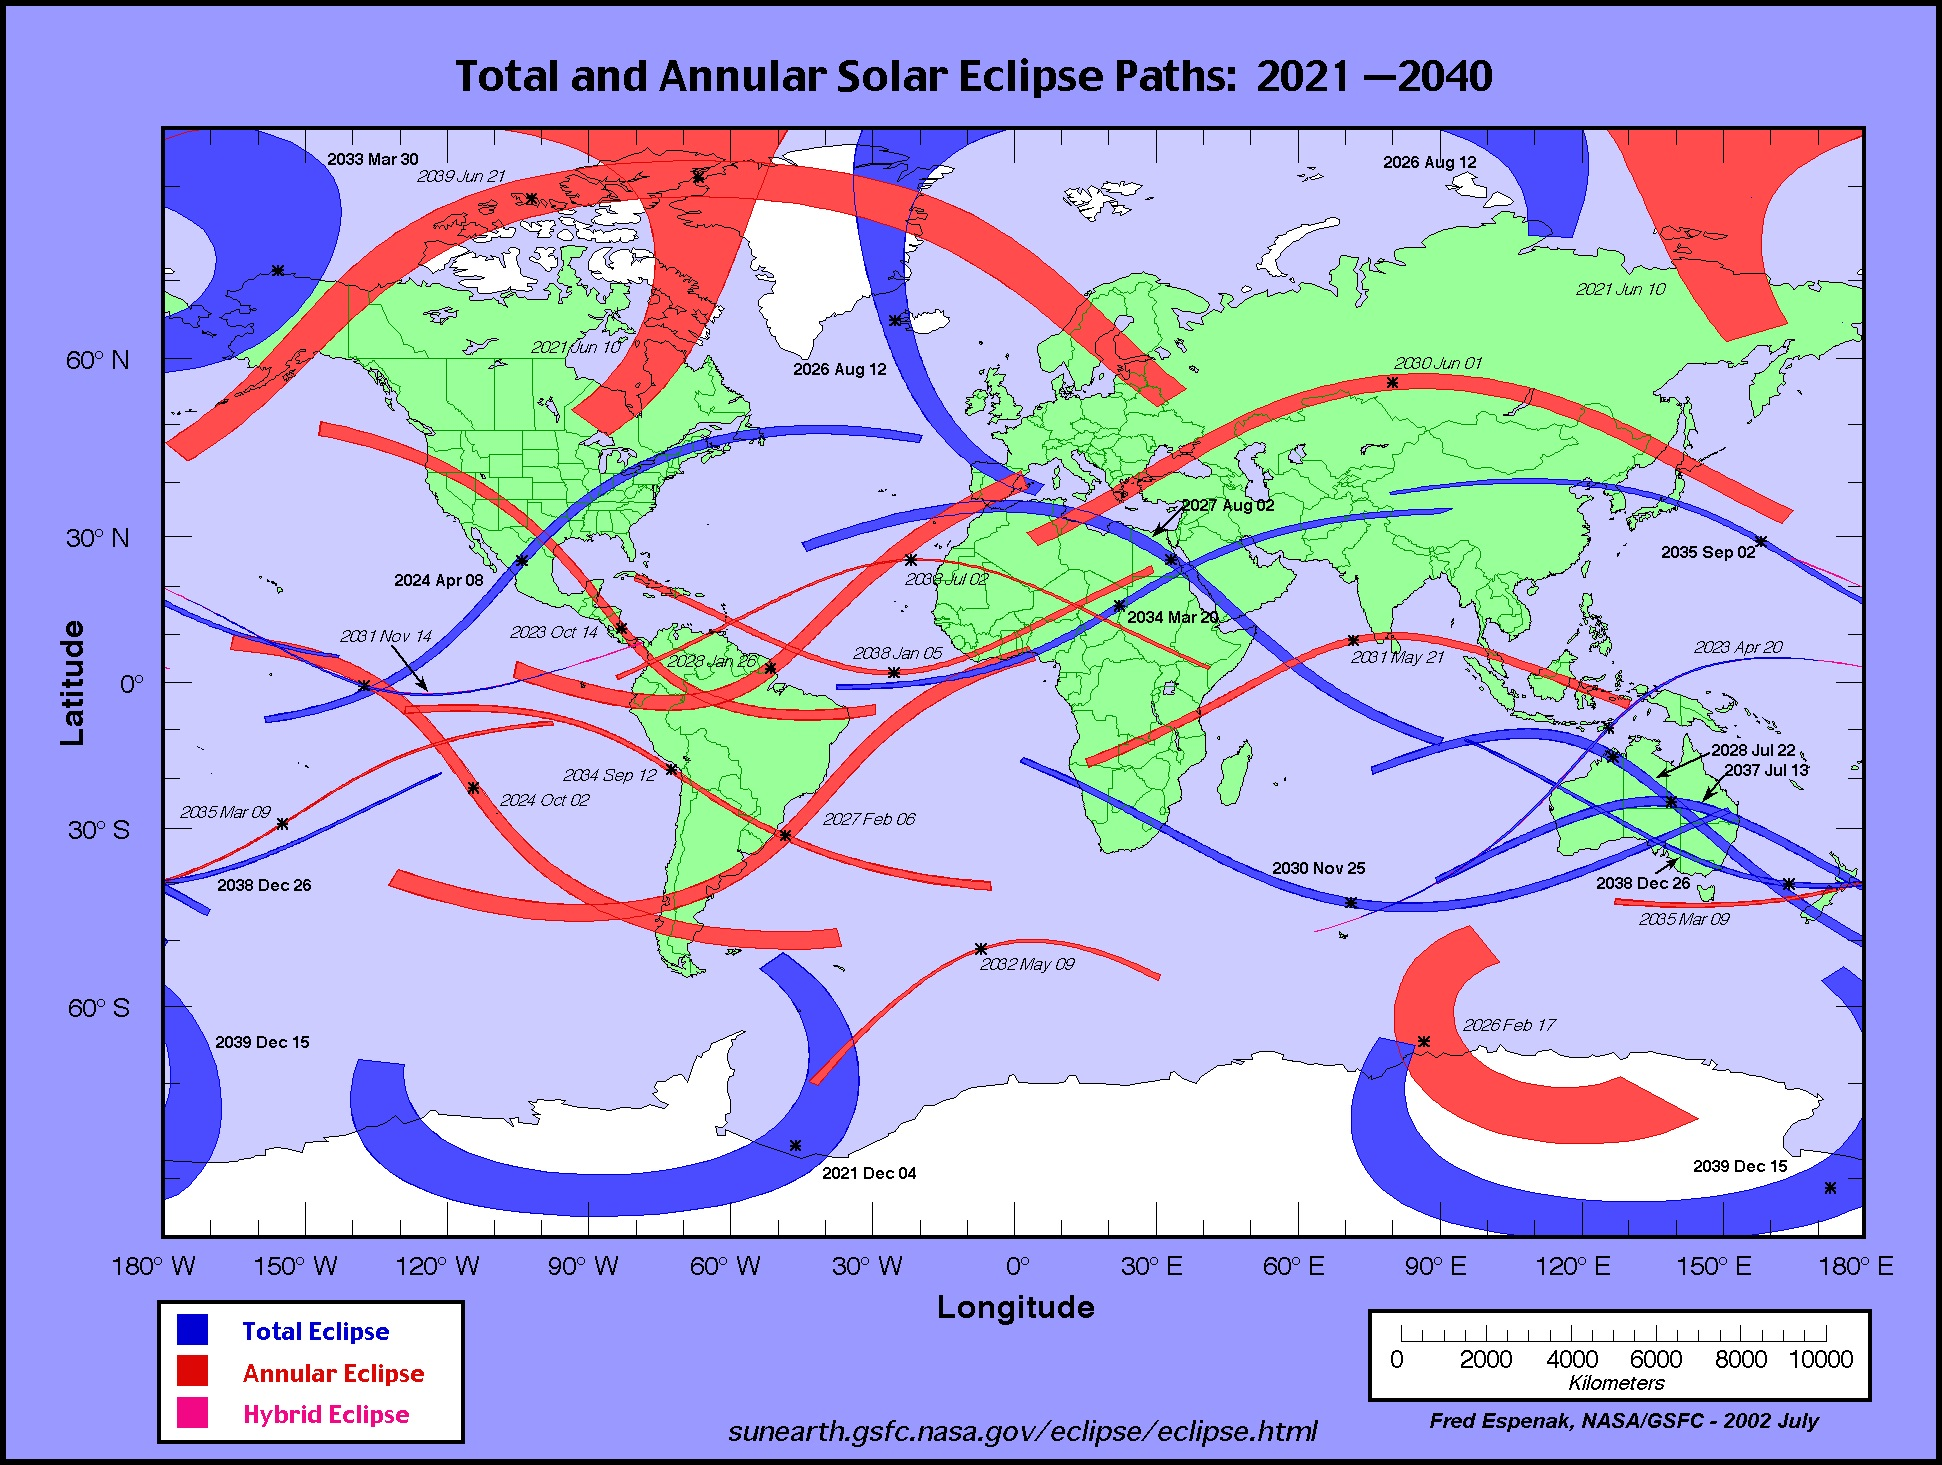
\includegraphics[scale=1]{Pictures/SEatlas2021.jpg}
\caption{Future eclipse paths}
\end{sidewaysfigure}

\subsection{Next Eclipse}
Next one in the area will be April 2024, but there will not be another total near by till after 2100....so do what you can to see this one.

\subsection{Safety}
\begin{itemize}
\item welding glasses...
\item Don't Look at Sun
\item etc
\end{itemize}

\subsection{What's going on in the Sky?}
\begin{itemize}
\item Saros cylce = 18 yrs, 11 days, 8 hrs.  (120degrees)
\item syzygy  "astronomical alignment"
	\begin{itemize}
\item 'all eclipses are syzygy events, but not all syzygy events are eclipses.'
	\end{itemize}
\end{itemize}

%\begin{figure} [!ht]
%\centering
%\includegraphics[width=85mm]{Figures/Hiperwall_overview.jpg}
%\caption{Hiperwall terminology/topology overview\citep{hiperwallmanual}}
%\label{fig:hp1}
%\end{figure}






\end{document}